\documentclass[a4paper]{article}
\usepackage[T1]{fontenc}
\usepackage[utf8]{inputenc}
\usepackage[italian]{babel}
\usepackage{graphicx}
\usepackage{listings}

\begin{document}


\author{Lorenzo Casini \and Sophia Fantoni}
\title{PROGRAMMAZIONE DI RETI \\ REPORT ASSIGNMENT 2}
\maketitle

\newpage

\tableofcontents	%per fare l'indice

\newpage

\section{Premessa}
Nel secondo assignment viene richiesto di implementare, a livello di trasporto, le funzioni lato receiver (A) e lato sender (B) utilizzando la tecnica Stop-and-Wait. A questo scopo è necessario, in primo luogo, comprendere a pieno il funzionamento del codice consegnatoci e successivamente implementare tale tecnica. 
\par La realizzazione del modello stop and wait non necessita di una coda di bufferizzazione in cui sono presenti i messaggi non ancora inviati. In un primo momento abbiamo seguito questa idea, ma ci siamo accorti che avevamo un'elevata perdita di pacchetti, in quanto il receiver, dopo aver inviato un pacchetto, non era in grado di memorizzare i successivi messaggi che riceveva fino alla recezione del primo ACK. Per questo motivo abbiamo deciso di bufferizzare all'interno di una coda tutti i messaggi ricevuti da A.

\section{Task 1}

\subsection{Struttura schematica del programma}
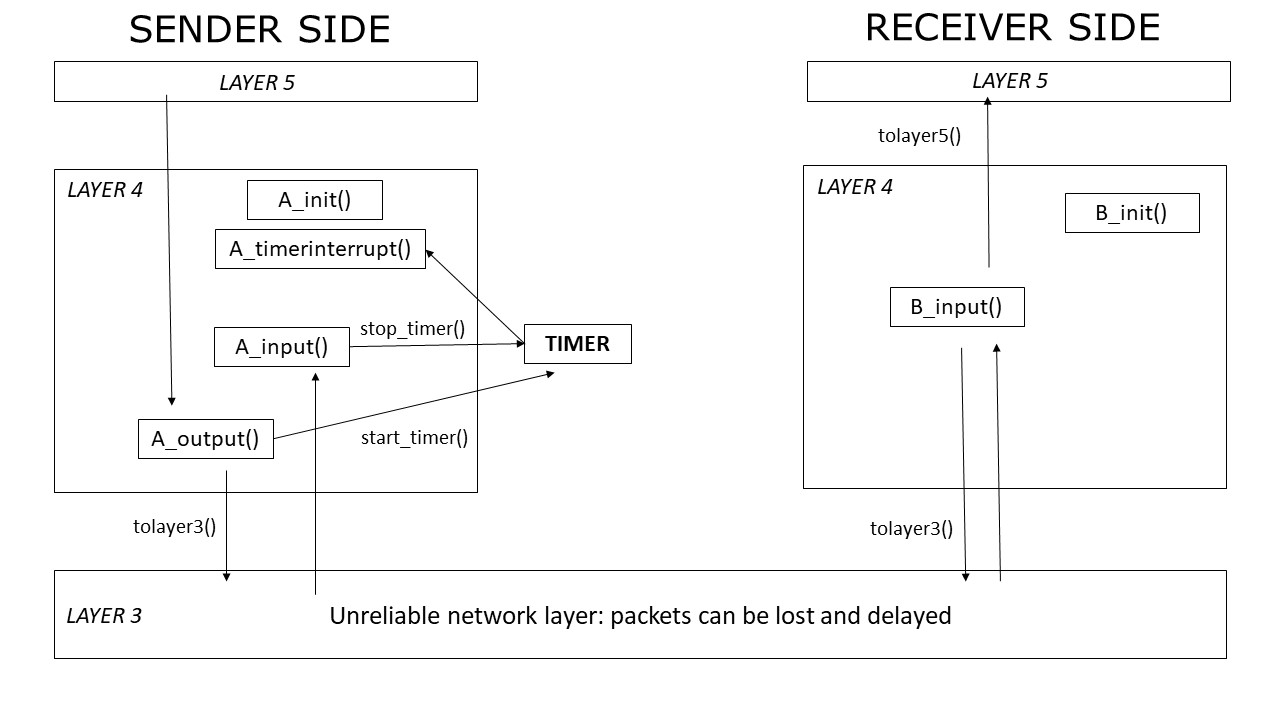
\includegraphics[width=\linewidth]{schema.jpg}

\subsection{Analisi del codice "netsimulator.c"}
Le prime funzioni che vengono eseguite effettuano l’inizializzazione delle variabili necessarie per l’invio e la recezione dei pacchetti sia lato sender che lato receiver, queste sono A\_init() e B\_init(). 
\par Quando il sender esprime il desiderio di inviare un messaggio al receiver, il layer 5 chiama la funzione A\_output(), essa si preoccupa di prendere il messaggio da inviare, inserirlo nel pacchetto e inizializzare gli altri valori. Successivamente, mediante la funzione tolayer3, invia il pacchetto al receiver e fa partire il timer con la funzione start\_timer(). Il lato sender rimane bloccato in attesa di recezione dell’ACK. 
\par Il livello 3 chiama la funzione B\_input() per indicare al receiver di riceve il pacchetto, esso ne controlla la correttezza, in caso positivo, invia il messaggio ricevuto correttamente al layer 5 e l’ACK al layer 3. 
\par Una volta che A riceve l’ACK, ne controlla l’integrità e, in caso positivo, ferma il timer. A questo punto il sender viene “sbloccato” e può eseguire l’invio di ulteriori messaggi. Allo scadere del timer viene chiamata la funzione A\_timerinterrup() che dovrà resettare il timer e rinviare il pacchetto perso o che è stato corrotto.



\section{Task 2}
\subsection{Analisi variabili e funzioni inserite}
Per implementare le funzioni richieste abbiamo dichiarato due variabili di tipo intero: seq\_number, variabile globale utilizzata per conoscere e controllare il numero di pacchetti inviati, e il valore ad esso successivo viene salvato in un’ulteriore variabile denominata next\_seq\_number. Inoltre, abbiamo dichiarato una costante per determinare se mostrare o no le informazioni di debug. Per bufferizzare i messaggi ricevuti dal sender A abbiamo creato la struttura Element che contiene il messaggio da inviare e il puntatore al successivo. Per controllare dove effettuare l’inserimento e l’eliminazione di elementi nella coda abbiamo dichiarato due puntatori al primo (first) e all’ultimo (last) elemento presente nella coda. Entrambi vengono inizializzati a NULL.  
\par La funzione calcChecksum ha il compito di calcolare il valore di checksum di ogni pacchetto. Tale numero sarà utilizzato nelle varie funzioni per verificare e gestire l’invio corretto di pacchetti. Il valore restituito è un intero, calcolato sommando il numero di sequenza, il valore di ack e i singoli caratteri contenuti nel payload.  Abbiamo deciso di sommare tutti questi valori in quanto risulti più probabile individuare l’errore, anche se questo è contenuto nel messaggio e nell’ack. 
\par La funzione isCorrupt viene richiamata per controllare se un pacchetto è stato corrotto. In caso negativo restituirà 0, in caso positivo un valore diverso da zero. 
\par Infine, le funzioni addqueue e dequeue si preoccupano rispettivamente di aggiungere un elemento nella lista e di eliminare un elemento dalla lista.

\subsection{Analisi delle funzioni da implementare}
\begin{flushleft}
\textbf{A\_init():} funzione che serve per inizializzare le variabili lato sender.
\end{flushleft}

\begin{flushleft}
\textbf{B\_init():} funzione che serve per inizializzare le variabili lato receiver.
\end{flushleft}

\begin{flushleft}
\textbf{A\_output(msg):}
 questo metodo viene chiamato dal layer 5. Esso prende in input il messaggio da inviare. Nel caso in cui il lato A abbia ricevuto un ACK dal lato B, tale messaggio verrà inserito all’interno del pacchetto e ne verranno inizializzati i diversi campi. Successivamente verrà chiamata la funzione tolayer3 che permette l’invio del pacchetto verso il receiver. Infine, viene fatto partire il timer e aggiornato il next\_seq\_number.
\end{flushleft}

\begin{flushleft}
\textbf{A\_input(pkt):} 
prende in input il pacchetto, viene chiamata dal layer 3 quando esso ha ricevuto il messaggio. Inizialmente si controlla la correttezza del pacchetto, nel caso in cui questo risulti corretto allora si ferma il timer ( stoptimer() ) e viene aggiornato il seq\_number. 
\end{flushleft}

\begin{flushleft}
\textbf{A\_timerinterrupt():} 
tale procedura viene chiamata nel momento in cui il timer scade. In tal caso sarà necessario rinviare il pacchetto chiamando la funzione tolayer3(), e far ripartire il timer.
\end{flushleft}

\begin{flushleft}
\textbf{B\_input(pkt): }
viene chiamata dal livello 3 quando il pacchetto arriva a B. Esso prende in input il pacchetto ricevuto, ne controlla l’integrità, inizializza i valori del pacchetto che contiene l’ACK. Infine, invia il messaggio a B, usando la funzione tolayer5 e invia l’ACK ad A chiamando tolayer3().
\end{flushleft}


\subsection{Modello a stati finiti}
Descrizione schematica del comportamento del receiver utilizzando una macchina a stati finiti.\par
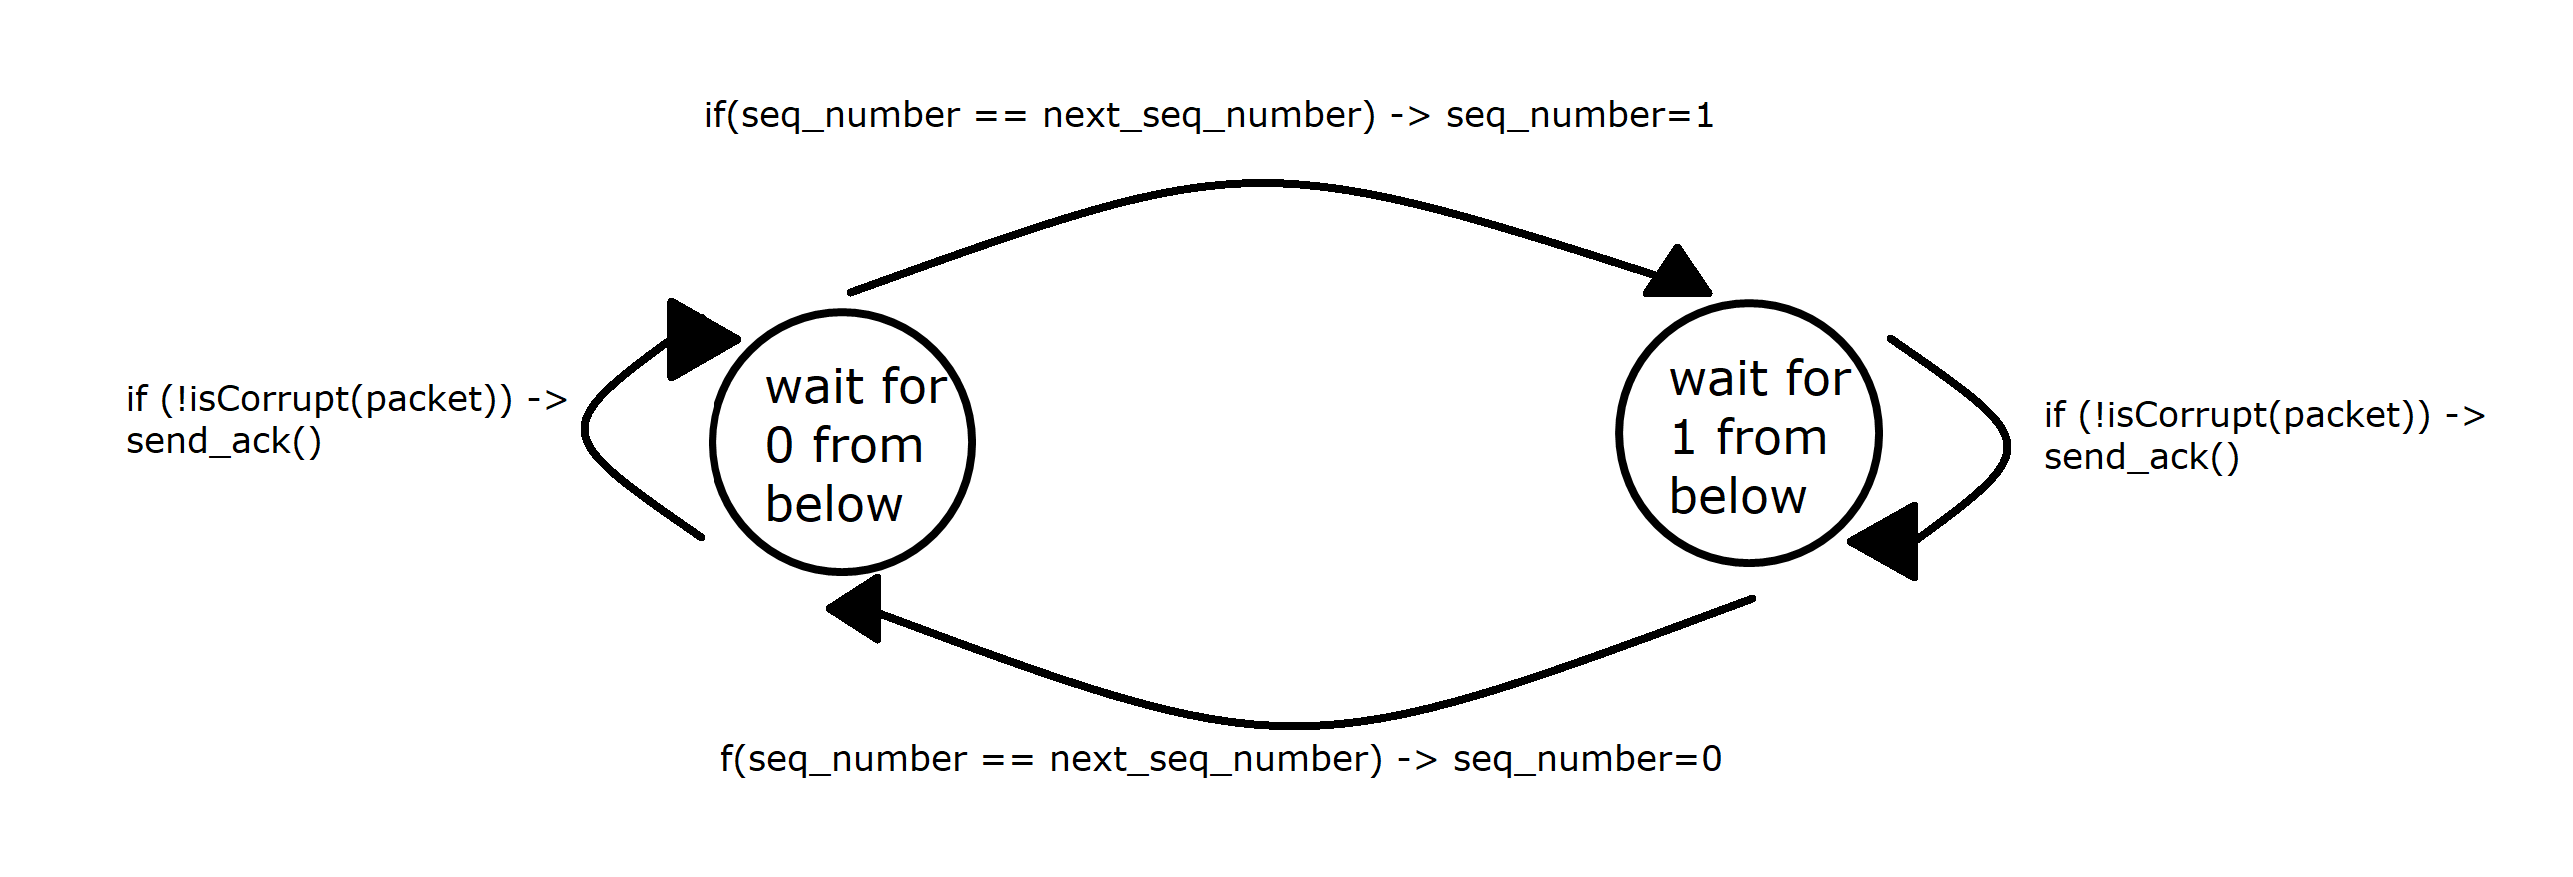
\includegraphics[width=\linewidth]{MSF.png}

\subsection{Test}
Visualizziamo il comportamento del nostro protocollo in due casi principali.
\paragraph{CASE 1} 
\par Analizziamo ora il caso in cui impostiamo i valori che indicano la perdita e la corruzione del pacchetto a 0 Inviamo xxxxx messaggi, il tempo medio dei messaggi dal livello 5 lato sender è 10, il timeout è 20, il trace level 2 e il random seed 2233.
\par Il lato A invia un pacchetto a B e si mette in attesa di ricevere l’ACK, 
la recezione e l’invio di ogni ulteriore pacchetto rimane bloccato finché non viene registrata la recezione dell’ACK. Il lato B attende di ricevere il pacchetto, successivamente invia l’ACK ad A e aggiorna il seq\_number.

\begin{lstlisting}[
    basicstyle=\scriptsize 
]
EVENT time: 0.554216,  type: 1, fromlayer5  entity: 0
A: Sending new DATA to B...
####[DEBUG]
 Seq number 0
 ACK number: 0
 Payload aaaaaaaaaaaaaaaaaaa
 Size: 20
 Checksum: 1843
####[DEBUG]

EVENT time: 2.053285,  type: 2, fromlayer3  entity: 1
B: Receiving DATA from A...
####[DEBUG]
 Seq number 0
 ACK number: 0
 Payload aaaaaaaaaaaaaaaaaaa
 Size: 20
 Checksum: 1843
####[DEBUG]
B: Checking packet checksum
B: Checksum OK!
B: Sending DATA to layer5
B: Sending ACK to A

EVENT time: 9.690878,  type: 2, fromlayer3  entity: 0
A: Receiving ACK from B...
A: Checking checksum ...
A: Checksum OK !
####[DEBUG]
 Seq number 0
 ACK number: 0
 Payload 000000000000000000
 Size: 20
 Checksum: 911
####[DEBUG]

EVENT time: 14.481033,  type: 1, fromlayer5  entity: 0
A: Sending new DATA to B...
####[DEBUG]
 Seq number 1
 ACK number: 1
 Payload bbbbbbbbbbbbbbbbbbb
 Size: 20
 Checksum: 1864
####[DEBUG]

EVENT time: 18.362560,  type: 2, fromlayer3  entity: 1
B: Receiving DATA from A...
####[DEBUG]
 Seq number 1
 ACK number: 1
 Payload bbbbbbbbbbbbbbbbbbb
 Size: 20
 Checksum: 1864
####[DEBUG]
B: Checking packet checksum
B: Checksum OK!
B: Sending DATA to layer5
B: Sending ACK to A

EVENT time: 20.381848,  type: 2, fromlayer3  entity: 0
A: Receiving ACK from B...
A: Checking checksum ...
A: Checksum OK !
####[DEBUG]
 Seq number 1
 ACK number: 1
 Payload 000000000000000000
 Size: 20
 Checksum: 913
####[DEBUG]

EVENT time: 20.730613,  type: 1, fromlayer5  entity: 0
A: Sending new DATA to B...
####[DEBUG]
 Seq number 2
 ACK number: 0
 Payload ccccccccccccccccccc
 Size: 20
 Checksum: 1883
####[DEBUG]

EVENT time: 25.962401,  type: 2, fromlayer3  entity: 1
B: Receiving DATA from A...
####[DEBUG]
 Seq number 2
 ACK number: 0
 Payload ccccccccccccccccccc
 Size: 20
 Checksum: 1883
####[DEBUG]
B: Checking packet checksum
B: Checksum OK!
B: Sending DATA to layer5
B: Sending ACK to A

EVENT time: 28.197302,  type: 2, fromlayer3  entity: 0
A: Receiving ACK from B...
A: Checking checksum ...
A: Checksum OK !
####[DEBUG]
 Seq number 2
 ACK number: 0
 Payload 000000000000000000
 Size: 20
 Checksum: 913
####[DEBUG]
\end{lstlisting}

\newpage

\paragraph{CASE 2}
Consideriamo il caso in cui vengono inviati in modo corretto 20 messaggi dal lato sender al receiver. Impostiamo il timeout, impostiamo il seme per settare i valori randomici a 2233, la probabilità di corruzione a 0.2, il trace level a 2 e il tempo medio a 10.

\begin{lstlisting}[
    basicstyle=\scriptsize 
]
EVENT time: 0.554216,  type: 1, fromlayer5  entity: 0
A: Sending new DATA to B...
####[DEBUG]
 Seq number 0
 ACK number: 0
 Payload aaaaaaaaaaaaaaaaaaa
 Size: 20
 Checksum: 1843
####[DEBUG]

EVENT time: 2.053285,  type: 2, fromlayer3  entity: 1
B: Receiving DATA from A...
####[DEBUG]
 Seq number 0
 ACK number: 0
 Payload aaaaaaaaaaaaaaaaaaa
 Size: 20
 Checksum: 1843
####[DEBUG]
B: Checking packet checksum
B: Checksum OK!
B: Sending DATA to layer5
B: Sending ACK to A

EVENT time: 9.690878,  type: 2, fromlayer3  entity: 0
A: Receiving ACK from B...
A: Checking checksum ...
A: Checksum OK !
####[DEBUG]
 Seq number 0
 ACK number: 0
 Payload 000000000000000000
 Size: 20
 Checksum: 911
####[DEBUG]

EVENT time: 14.481033,  type: 1, fromlayer5  entity: 0
A: Sending new DATA to B...
####[DEBUG]
 Seq number 1
 ACK number: 1
 Payload bbbbbbbbbbbbbbbbbbb
 Size: 20
 Checksum: 1864
####[DEBUG]

EVENT time: 18.362560,  type: 2, fromlayer3  entity: 1
B: Receiving DATA from A...
####[DEBUG]
 Seq number 1
 ACK number: 1
 Payload bbbbbbbbbbbbbbbbbbb
 Size: 20
 Checksum: 1864
####[DEBUG]
B: Checking packet checksum
B: Checksum OK!
B: Sending DATA to layer5
B: Sending ACK to A

EVENT time: 20.381848,  type: 2, fromlayer3  entity: 0
A: Receiving ACK from B...
A: Checking checksum ...
A: Checksum OK !
####[DEBUG]
 Seq number 1
 ACK number: 1
 Payload 000000000000000000
 Size: 20
 Checksum: 913
####[DEBUG]

EVENT time: 20.730613,  type: 1, fromlayer5  entity: 0
A: Sending new DATA to B...
####[DEBUG]
 Seq number 2
 ACK number: 0
 Payload ccccccccccccccccccc
 Size: 20
 Checksum: 1883
####[DEBUG]

EVENT time: 25.962401,  type: 2, fromlayer3  entity: 1
B: Receiving DATA from A...
####[DEBUG]
 Seq number 2
 ACK number: 0
 Payload ccccccccccccccccccc
 Size: 20
 Checksum: 1883
####[DEBUG]
B: Checking packet checksum
B: Checksum OK!
B: Sending DATA to layer5
B: Sending ACK to A

EVENT time: 28.197302,  type: 2, fromlayer3  entity: 0
A: Receiving ACK from B...
A: Checking checksum ...
A: Checksum OK !
####[DEBUG]
 Seq number 2
 ACK number: 0
 Payload 000000000000000000
 Size: 20
 Checksum: 913
####[DEBUG]

EVENT time: 28.612934,  type: 1, fromlayer5  entity: 0
          TOLAYER3: packet being lost
A: Sending new DATA to B...
####[DEBUG]
 Seq number 3
 ACK number: 1
 Payload ddddddddddddddddddd
 Size: 20
 Checksum: 1904
####[DEBUG]

EVENT time: 48.612934,  type: 0, timerinterrupt   entity: 0
A: Timer Interrupt !
A: Resending latest packet ...

EVENT time: 52.672170,  type: 2, fromlayer3  entity: 1
B: Receiving DATA from A...
####[DEBUG]
 Seq number 3
 ACK number: 1
 Payload ddddddddddddddddddd
 Size: 20
 Checksum: 1904
####[DEBUG]
B: Checking packet checksum
B: Checksum OK!
B: Sending DATA to layer5
B: Sending ACK to A

EVENT time: 54.556871,  type: 2, fromlayer3  entity: 0
A: Receiving ACK from B...
A: Checking checksum ...
A: Checksum OK !
####[DEBUG]
 Seq number 3
 ACK number: 1
 Payload 000000000000000000
 Size: 20
 Checksum: 915
####[DEBUG]
\end{lstlisting}


\end{document}